\documentclass[crop=false]{standalone}
% --- ПРЕАМБУЛА ДЛЯ ПОДДЕРЖКИ РУССКОГО ЯЗЫКА И МАТЕМАТИКИ ---
\usepackage[T2A]{fontenc}
\usepackage[utf8]{inputenc}
\usepackage[russian]{babel}
\usepackage{amsmath}
\usepackage{geometry}
\usepackage{amssymb}
\usepackage{graphicx}
\usepackage{float}
\usepackage{import}
\geometry{a4paper, top=2cm, bottom=2cm, left=2cm, right=2cm}
\newcommand{\sidecomment}[1]{\marginpar{\raggedright\scriptsize\itshape #1}}
\newcommand{\iu}{\mathrm{i}}

\newcommand{\Def}{%
    \text{Def}%
    \hspace{-0.85em}% Сдвиг назад ровно на середину (подберите под шрифт)
    \raisebox{0.1ex}{/}% Черта
    \hspace{1em}% Возврат к концу слова + небольшой отступ
}

\renewcommand{\Re}{\operatorname{Re}}
\renewcommand{\Im}{\operatorname{Im}}

\ifstandalone
    \newcommand{\lecturebreak}{} % В отдельном файле лекции разрыв не нужен
\else
    \newcommand{\lecturebreak}{\clearpage} % В полной книге - начинаем с новой страницы
\fi

\newcounter{lecturenumber} % Создаем счетчик для нумерации лекций
\newcommand{\lecture}[2]{
    \lecturebreak
    \refstepcounter{lecturenumber} % Увеличиваем счетчик на 1
    \par\vspace{2em}\noindent % Отступ сверху и убираем абзацный отступ
    {\Large\bfseries % Делаем заголовок крупным и жирным
    Лекция \thelecturenumber: #1 % Выводим "Лекция N: Тема"
    \hfill % Растягиваем пробел, чтобы дата была справа
    \large\textit{#2}} % Выводим дату курсивом
    \par\vspace{1em} % Небольшой отступ снизу
    \addcontentsline{toc}{section}{Лекция \thelecturenumber: #1} % Добавляем в оглавление
    \par
}

\newcommand{\TwoCols}[2]{%
  \par\noindent % Начать с новой строки без отступа
  \begin{minipage}[t]{0.48\textwidth}
    #1
  \end{minipage}% <-- Важный '%' для удаления пробела
  \hfill % Растягивающийся пробел между колонками
  \begin{minipage}[t]{0.48\textwidth}
    #2
  \end{minipage}% <-- Важный '%' для удаления пробела
  \par%
}

\pagestyle{plain} % Включаем нумерацию страниц\
\begin{document}
\lecture{}{08.06}
\section{Исследование динамических уравнений Эйлера}
\[
\begin{cases}
    A \dot p + q r (C - B) = M_{O x} \\
    B \dot q + p r (A - C)= M_{O y} \\
    C \dot r + p q ( B - A) = M_{O z}
\end{cases}
\]
В случае Эйлера:
\begin{enumerate}
     \setcounter{enumi}{-1}
    \item Нет движения
    \[p = q = r = 0\]
    \item 
    Стационарное вращение
    \[p = \text{ const } \qquad q =\text{ const } \qquad r = \text{ const }\]
    Когда тело будет продолжать вращаться вокруг изначальной оси?
    \[\begin{cases}
        q r (C - B) = 0,\\
        p r ( A - C) = 0, \\
        pq (B - A) = 0
    \end{cases}\]
    \begin{enumerate}
        \item Например Шар/Куб \[A = B = C\]
        Не зависит от оси

        \item
        \[A = B \neq C \implies r = 0 \; \| \; p = q = 0\]
        Вращение вокруг оси в плоскости $Oxy$, либо вращение вокруг оси перпендикулярной $Oxy$
        \[A \neq B \; \&  \; B \neq C  \; \& \; A \neq C \implies \text{ хотя бы одна пара из проекций угловой скорсти равна нулю}\]
        Вращение вокруг координатных осей
    \end{enumerate}
    \item 
    Регулярная прецессия динамически симметричного($A = B \; \&\; C \neq 0$) твёрдого тела
    \[\begin{cases}
        \dot p A + q r( C - A) = 0, \\
        \dot q B + p r ( A - C) = 0, \\
        \dot r C = 0
    \end{cases} \implies r = r_0 = \text{ const}\]
    \[
    \begin{dcases}
        C r = K_{O_{z'}} = K_O \cos \theta = \text{ const} \\
        A p = K_{O_{x'}} = K_O \sin \theta \sin \varphi,  \\ 
        A q = K_{O_{y'}} = K_O \sin \theta \cos \varphi \end{dcases} 
    \implies
     \begin{dcases} 
        K_O = \frac{C r_0}{\cos \theta}, \\ 
        \theta = \theta_0 = \arccos \frac{C r_0}{K_O} = \text{ const} \\
        p = \frac{K_O}{A}\sin \theta \sin \varphi,\\
     q = \frac{K_O}{A} \sin \theta \cos \varphi
    \end{dcases}
     \]
    \begin{figure}[H]
    \centering
    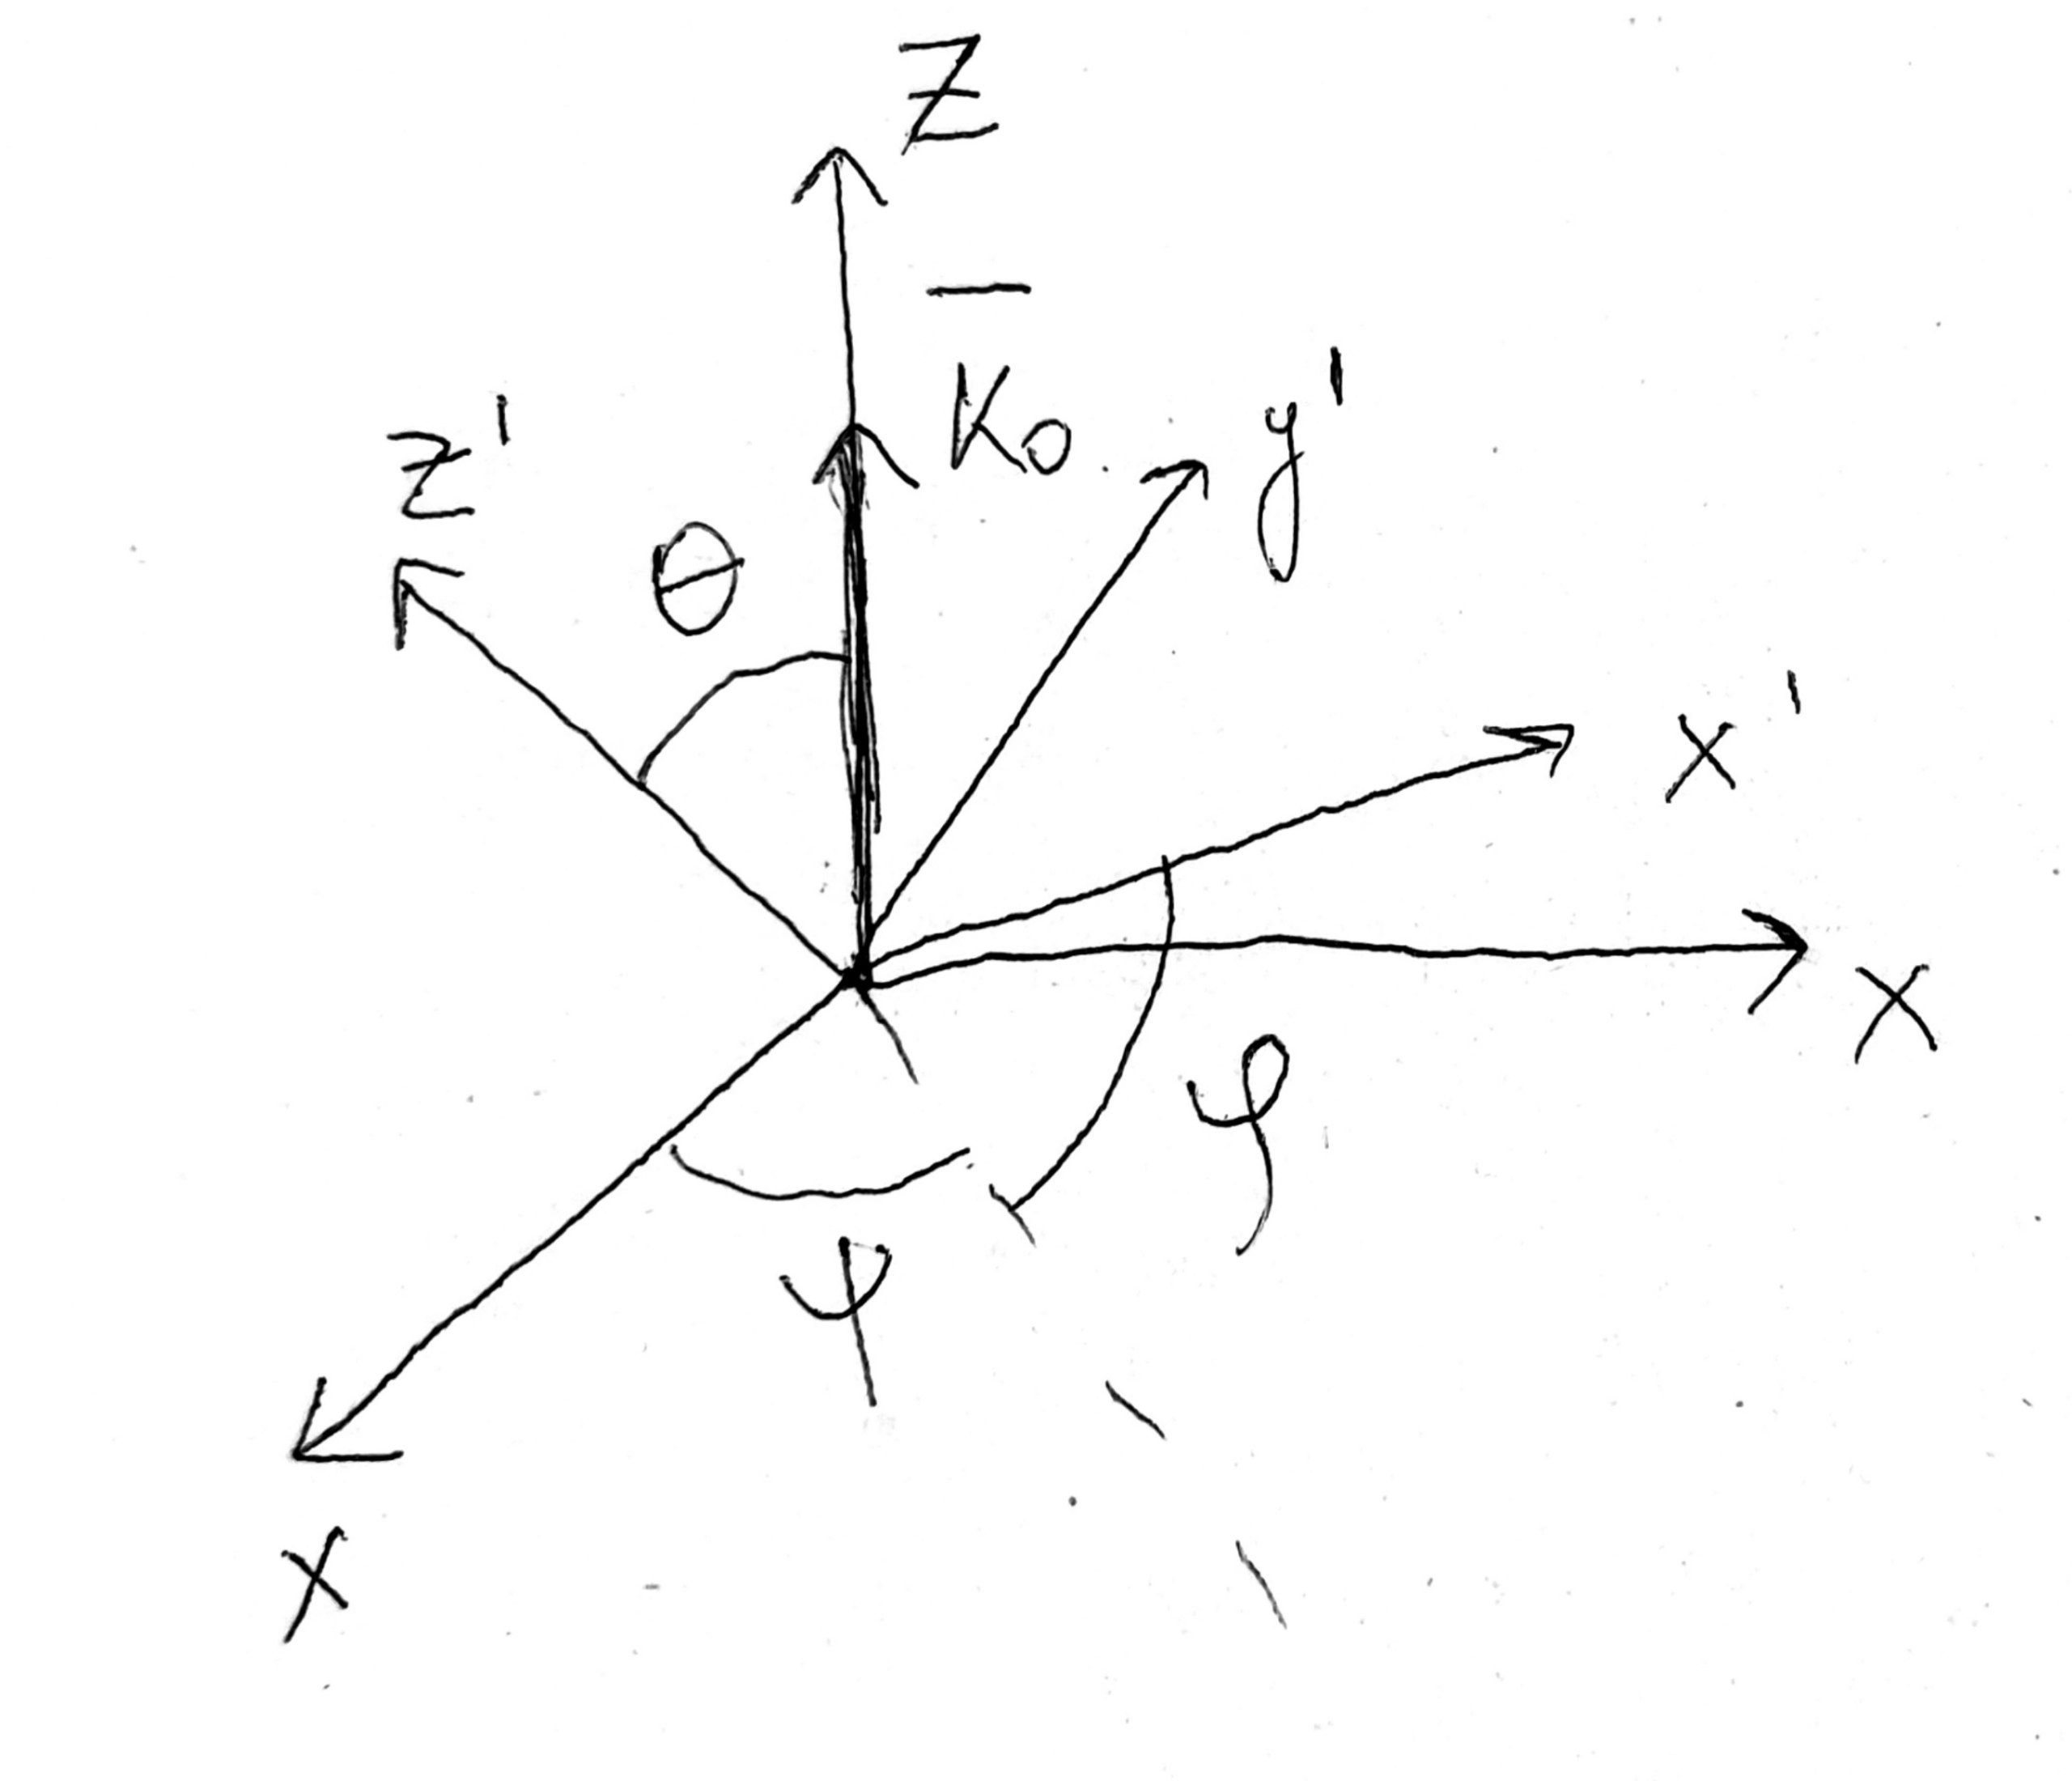
\includegraphics[width=0.5\textwidth]{KOProjections.jpg}
    \caption{}
    \label{fig:myimage} 
    \end{figure}
    \[
    \begin{dcases}
    p = \dot \psi \sin \theta_0 \sin \varphi = \frac{K_O}{A} \sin \theta_0 \sin \varphi \\ q = \dot \psi \sin \theta_0 \cos \varphi = \frac{K_O}{A} \sin \theta_0 \cos \varphi \\ r = \dot \psi \cos \theta_0 + \dot \varphi
    \end{dcases} \implies \begin{dcases}
        \dot \psi = \frac{K_O}{A}, \\
        \begin{aligned}
            \dot \varphi &= r - \dot \psi \cos \theta_0 = \frac{K_O}{C} \cos \theta_0 - \frac{K_O}{A} \cos \theta_0 \\ &= K_O \cos \theta_0 \left(\frac{A - C}{C A} \right) = r_0 \frac{A - C}{A}
        \end{aligned}
    \end{dcases}
    \]
    \[
    \boxed{
    \begin{dcases}
    \dot \varphi = r_0 \cdot \frac{A- C}{A}, \\
    \dot \psi = \frac{K_O}{A}, \\ 
    \theta_0 = \text{ const} & \cos \theta_0 = \frac{C}{K_O} \cdot r_0  \\
    \end{dcases}
    }
    \]
    То есть если раскрутить тело не вокруг главной оси инерции, то оно начинает прецессировать
    
    Эти формулы описывают движение точки, в которой ось инерции протыкает Землю(Угловая скорость нуль), вокруг географическиого полюса Земли

    Но на самом деле с Землёй всё сложнее, возникают Чандлеровские колебания
\end{enumerate}
\section{Геометрическая интерпретация Пуансо}
\begin{figure}[H]
    \centering
    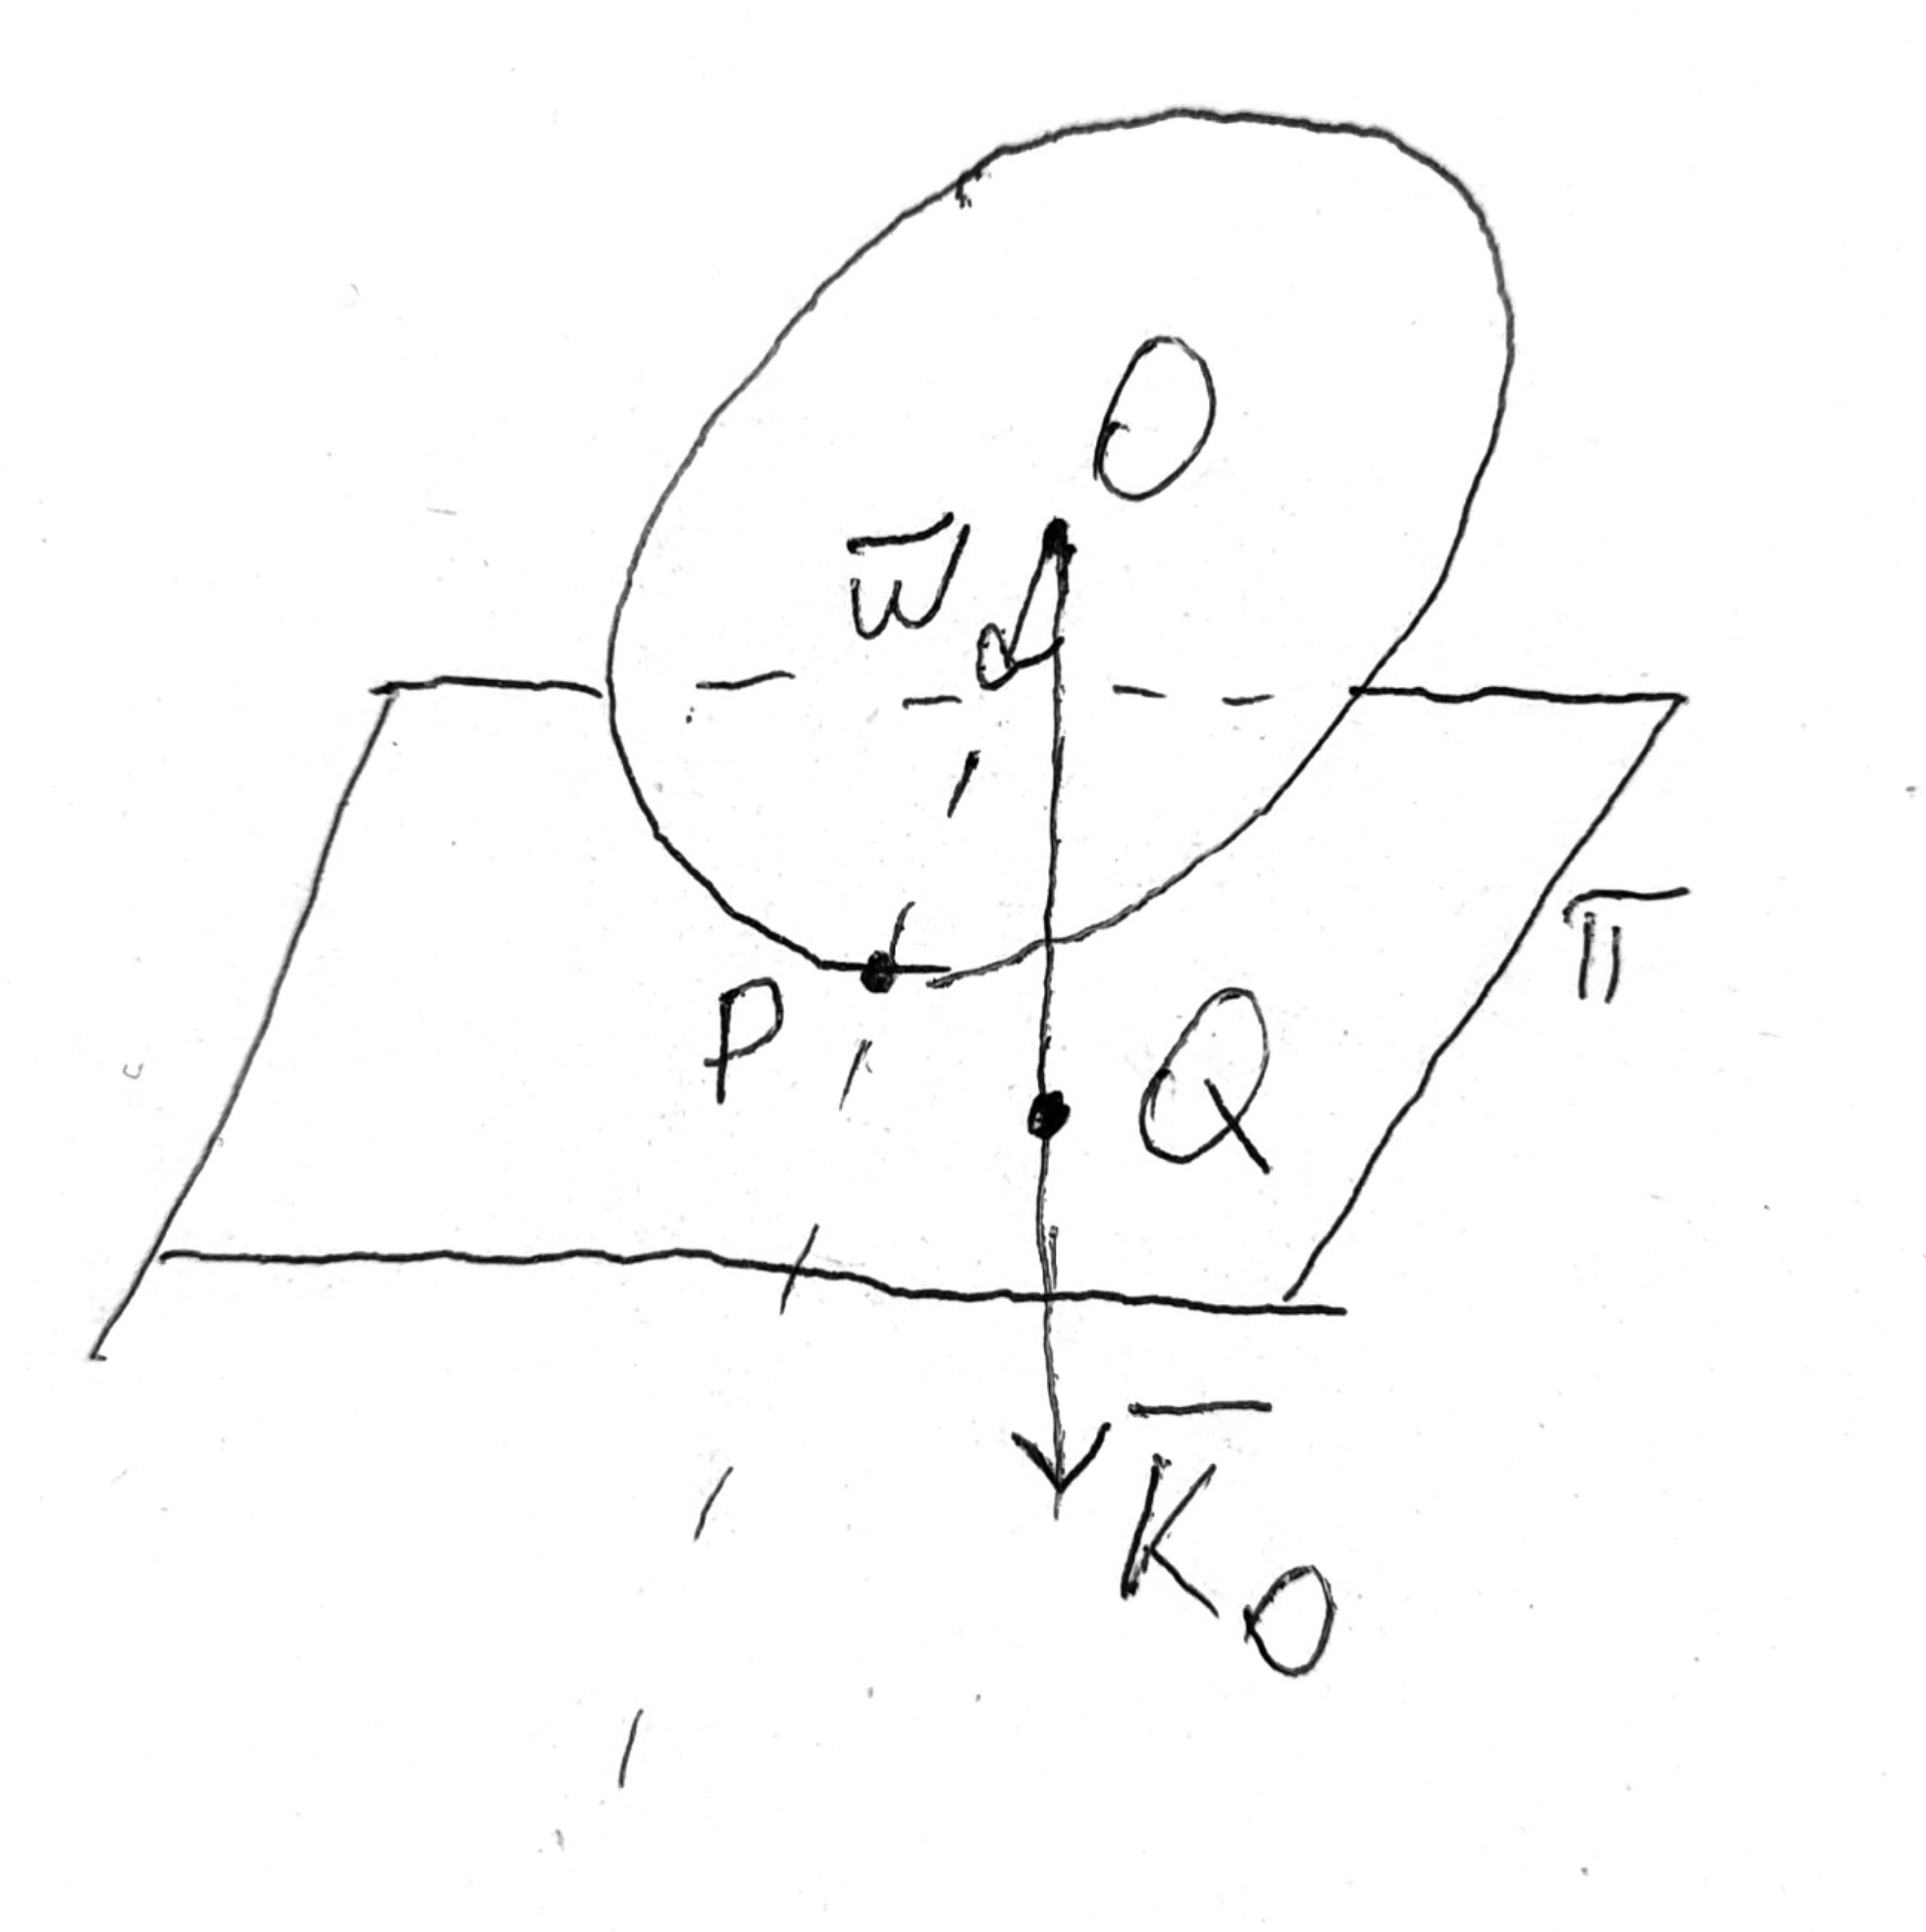
\includegraphics[width=0.4\textwidth]{precession.jpg}
    \caption{}
    \label{fig:myimage} 
    \end{figure}
\[: \pi \perp \bar K_O \qquad \overline{OP} = \lambda \bar \omega\]
\begin{enumerate}
    \item $\pi$ — касательная к эллипсоиду плоскость в точке $P$
    \begin{proof}
    \[\bar n = \nabla (x^2 A + y^2 B + z^2 C) = \begin{pmatrix}
        2 A x \\ 2 B y \\ 2 C z
    \end{pmatrix} = 2 \lambda \begin{pmatrix}
        A p \\ B q \\ C r
    \end{pmatrix} = 2 \lambda \bar K_O\]
\end{proof}
    \item \[OQ = \frac{\sqrt{2 T}}{K_O}\]
    \begin{proof}
        \[OQ = \frac{(\bar OP, \bar K_O)}{K_O} = \frac{A x p + B y q + C z r}{\sqrt{A^2 p^2 + B^2 q^2 + C^2 r^2}} = \frac{\lambda (A p^2 + B q^2 + C r^2)}{K_O} = \frac{\frac{1}{\sqrt{2 T}} 2 T}{K_O} = \frac{\sqrt{2 T}}{K_O}\]
    \end{proof}
    \item 
    \[\lambda = \frac{1}{\sqrt{2 T}}\]
    \begin{proof}
        \[\bar OP = \lambda \bar \omega \qquad \begin{pmatrix}
            x \\ y \\ z
        \end{pmatrix} = \begin{pmatrix}
            \lambda p \\ \lambda q \\ \lambda r
        \end{pmatrix} \qquad x^2 A + y^2 B + z^2 C = 1\]
        \[\lambda^2 (p^2 A + q^2 B + r^2 C) = \lambda^2 2 T = 1 \implies \lambda = \frac{1}{\sqrt{2 T}}\]
    \end{proof}
\end{enumerate}
\noindent \keypoint При вращении точка $P$ будет заметать полоиду(не обязательно окружность)

Художественный талант и лень автора не позволили ему нарисовать собственную рисунок, рисунок Сергея Алексеевича и рисунок с просторов Интернета:
\begin{figure}[H]
    \centering
    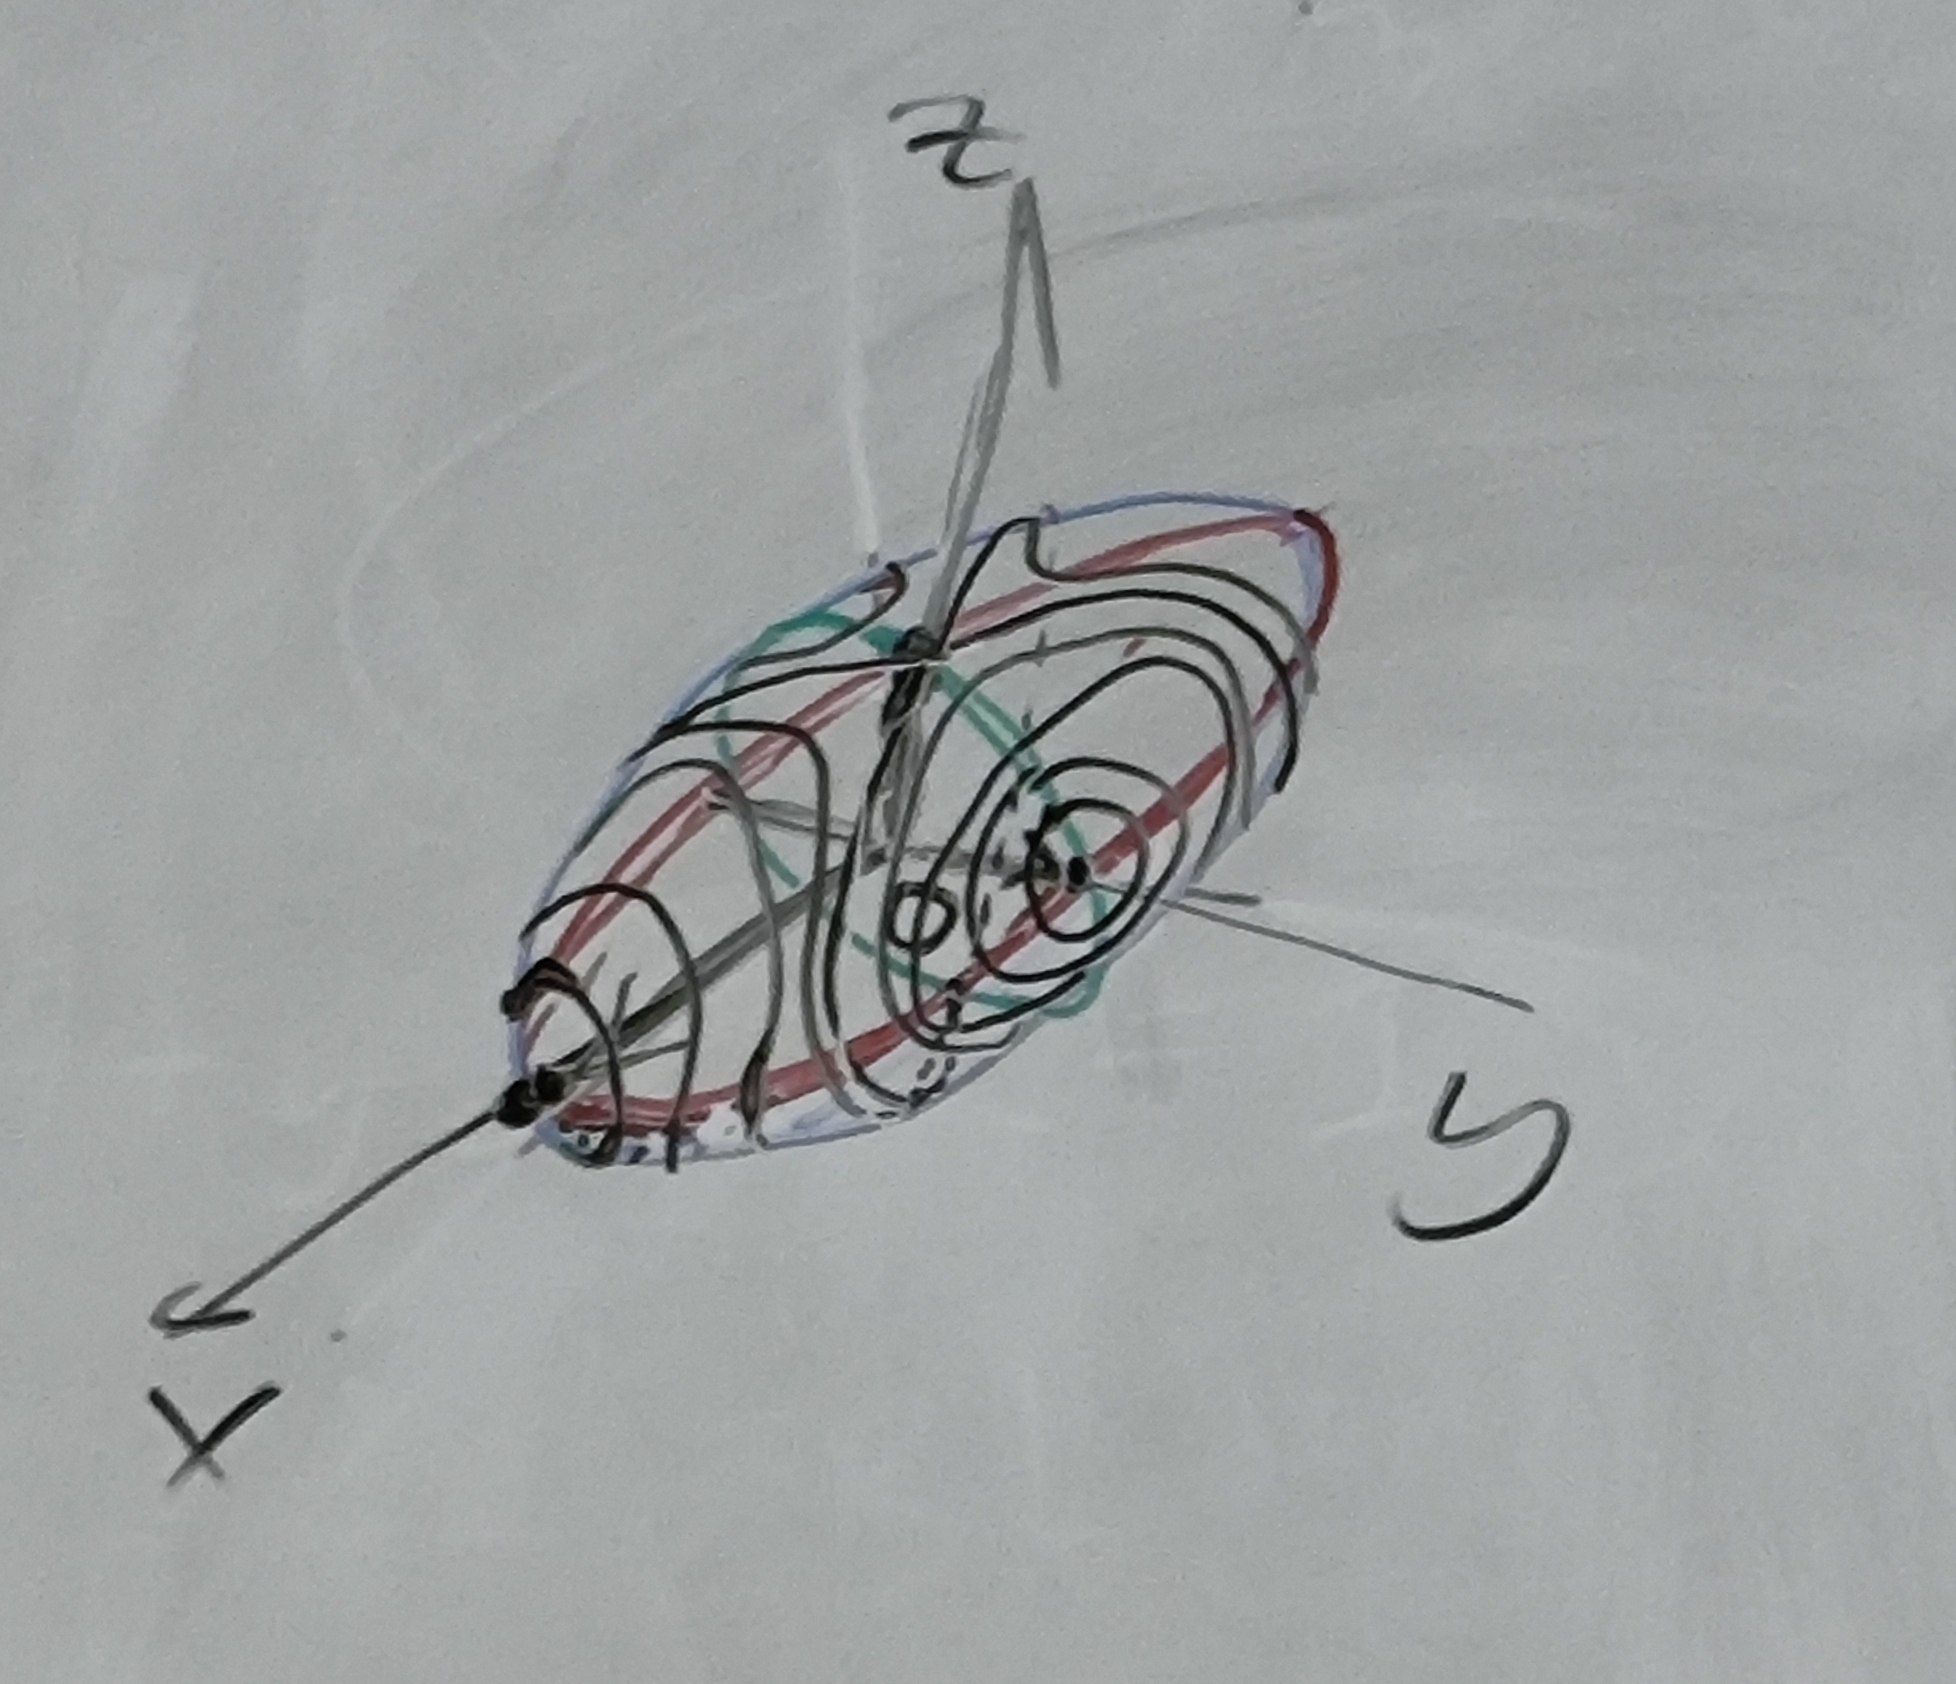
\includegraphics[width=0.3\textwidth]{aks.jpg}
    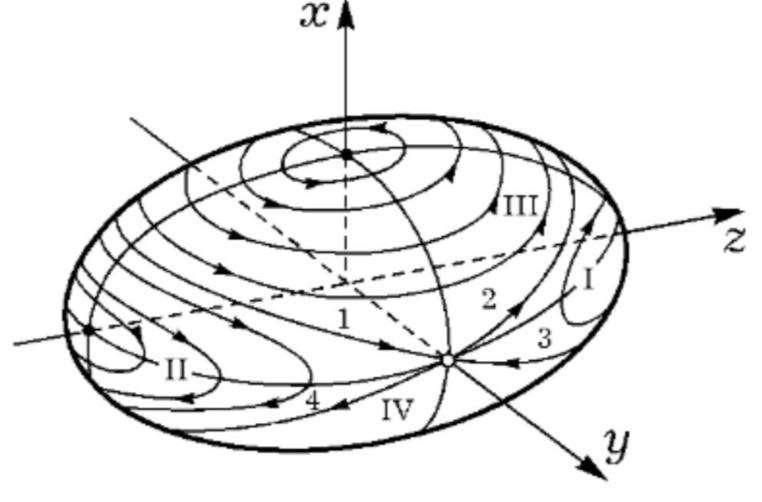
\includegraphics[width=0.3\textwidth]{web.jpg} %fixme будто съехало
    \caption{}
    \label{fig:myimage} 
    \end{figure}

\noindent \keypoint Замечание: как бы аккуратно не раскручивали тело, вокруг $z$ вращаться не будет, так как седло — положение неусточивое, то есть если твёрдое тело раскрутить вокруг оси соответствующей среднему моменту инерции, то угловая скорость начнёт периодически менять своё направление(Эффект Джанибеков)

\noindent \keypoint Что не успели в курсе:
\begin{itemize}
    \item 
    Элементарная теория гироскопа
    \item
    формула вынужденной прецессии твердого тела
    \item
    Задача двух тел, Законы Кеплера
\end{itemize}
\end{document}